\documentclass[11pt]{article}
\usepackage[T1]{fontenc}
\usepackage[utf8]{inputenc}
\usepackage[USenglish,british,american,australian,english]{babel}
\usepackage{graphicx}
\usepackage{subcaption}
\usepackage{float}
\usepackage{hyperref}
\usepackage{amsmath}
\usepackage{listings}
\usepackage{xcolor}
\lstset{
	basicstyle=\fontsize{10}{11}\ttfamily\color{black},
	commentstyle=\ttfamily\color{red},
	keywordstyle=\ttfamily\color{blue},
	stringstyle=\color{orange},
	tabsize=2,
	numbers=left,
	numberstyle=\tiny,
	firstnumber=1,
	numberfirstline=false,
	frame=single,
	showstringspaces=false,
	inputencoding=utf8,
	breaklines=true,
	language=python,
}

\title{\textbf{Weather image classification} \\ \bigskip \large Homework 2 - Machine Learning \\ Engineering in Computer Science \\ "La Sapienza" University of Rome}
\author{Costa Marco 1691388}
\date{\today}

\begin{document}
\maketitle
\pagebreak
\tableofcontents
\pagebreak

\section{Introduction}
The purpose of this homework is to solve a \textit{multi-class} image classification problem on the \textbf{\textit{Multi-class Weather Image Dataset}}. The problem must be solved using two modes:
\begin{enumerate}
	\item Define a CNN and train it from scratch;
	\item Apply transfer learning and fine tuning from a pre-trained model.
\end{enumerate}
After that, we have to evaluate the two models in a proper way. The metrics used for the comparison of the models are the accuracy and the loss function (\textit{Categorical Crossentropy}).
Finally we have to perform a prediction on the \textbf{\textit{WeatherBlindTestSet}} and create a \textit{.csv} file in which there is the predicted label for each image.
Moreover, we have to provide a personal dataset made with our photos. 


\subsection{Dataset}
The \textbf{\textit{Multi-class Weather Image Dataset}} contains images grouped in four classes: \textbf{HAZE}, \textbf{RAINY}, \textbf{SNOWY}, \textbf{SUNNY}.
It is very balanced: the whole dataset has 1000 images for each class.
It is organized in a file system structure with four folders corresponding to the four classes \textit{HAZE}, \textit{RAINY}, \textit{SNOWY}, \textit{SUNNY} and containing the corresponding images.
In addition, there is the \textbf{\textit{SMART-I weather test set}} that can be used as test set. It contains only the three classes \textit{RAINY}, \textit{SNOWY}, \textit{SUNNY} and it is very unbalanced. 
Images in the datasets have different shapes and resolutions. It is necessary to reshape these images to make image dimensions consistent with the input layer of the network.
Finally there is the \textbf{\textit{WeatherBlindTestSet}} on which we have to perform the prediction with the best model.

\subsection{Hardware}
Since we use tensorflow and keras libraries, the performance (training time, prediction, etc.) depends on the hardware, and in particular on the GPU. We used the \textit{Nvidia GeForce GTX 950M}, having 640 \textit{CUDA cores}, 4Gb of \textit{DDR3 Memory} and 1000 MHz of clock.

\section{Define a CNN and train it from scratch}
Since defining a CNN is very difficult, I decided to use a known network, namely AlexNet, to have a comparison. All the nets were trained in 100 epochs, with the same image input dimension ($118 \times 224$), all the images were loaded in color mode ``\textit{RGB}'' with batch size 32 and data augmentation. My nets are named \textit{KucoNet v.x}.

\subsection{AlexNet}
Since \textit{AlexNet} is a well-known CNN, its definition isn't shown. \\
\textbf{Parameters}:
\begin{itemize}
	\item Total params: 28,083,756
	\item Trainable params: 28,062,620
	\item Non-trainable params: 21,136
\end{itemize}
\textbf{Results}:
\begin{itemize}
	\item Final epoch performances:
	\begin{itemize}
		\item Accuracy: 0.8122
		\item Loss: 0.8266
	\end{itemize}
	\item Test set performances
	\begin{itemize}
		\item Accuracy : 0.7320
		\item Loss: 0.9699
	\end{itemize}
	\item Training time: $\approx$ 1 hour and 5 minutes
\end{itemize}
\begin{figure}[H]
	\centering
	\begin{subfigure}[b]{0.4\linewidth}
		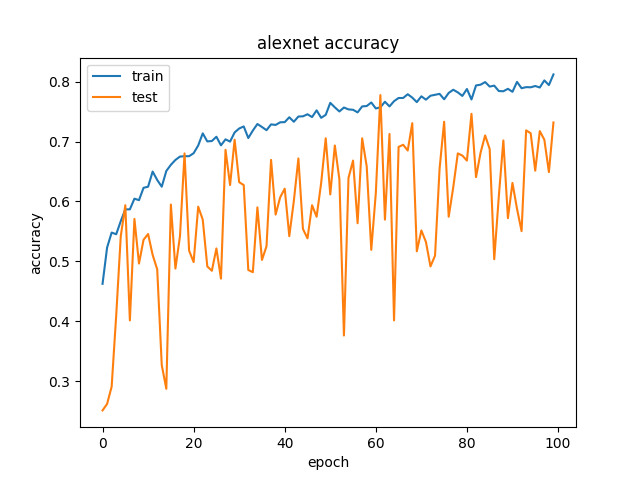
\includegraphics[width=\linewidth]{../images/alexnet_100_epochs_accuracy.png}
		\caption{Accuracy}
	\end{subfigure}
	\begin{subfigure}[b]{0.4\linewidth}
		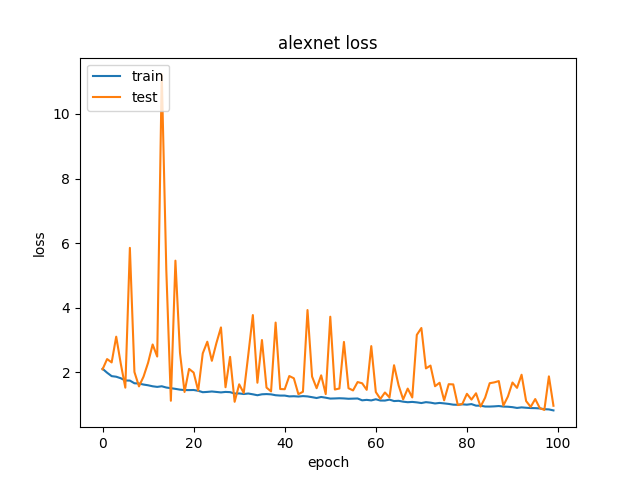
\includegraphics[width=\linewidth]{../images/alexnet_100_epochs_loss.png}
		\caption{Loss}
	\end{subfigure}
	\caption{AlexNet performaces plots}
	\label{fig:alexnetperformances}
\end{figure}

\subsection{KucoNet v.1}
The first CNN is defined as follow:
\begin{table}[H]
	\begin{center}
		\begin{tabular}{|l|r|}
			\hline
			\textbf{Layer (type)} & \textbf{Parameters} \\
			\hline
			Convolutional & 32, kernel $5 \times 5$ \\
			\hline
			Max Pooling & pool $2 \times 2$ \\
			\hline
			Convolutional & 64, kernel $3 \times 3$ \\
			\hline
			Max Pooling & pool $2 \times 2$ \\
			\hline
			Flatten & \\
			\hline
			Fully Connected & 1024 neurons  \\
			\hline
			Fully Connected & 4 neurons \\
			\hline 
		\end{tabular}
	\end{center}
\end{table} 
The first convolutional layer produces 32 feature maps using a $5 \times 5$ kernel followed by max-pooling operation. The second convolutional layer produces 64 feature maps using a $3 \times 3$ kernel followed by a max-pooling operation. After that, feature maps are sent to the dense layer, which includes 1024 neurons. Finally, the last layer is a dense layer  composed by 4 neurons that produces the output. The activation function is \textit{relu} for all the layers, except the last one that uses \textit{softmax}. The model is compiled with the \textit{Adam} optimizer and the \textit{categorical\_crossentropy} loss function. \\
\textbf{Parameters}:
\begin{itemize}
	\item Total params: 95,577,540
	\item Trainable params: 95,577,540
	\item Non-trainable params: 0
\end{itemize}
\textbf{Results}:
\begin{itemize}
	\item Final epoch performances:
	\begin{itemize}
		\item Accuracy: 0.8066
		\item Loss: 0.5284
	\end{itemize}
	\item Test set performances
	\begin{itemize}
		\item Accuracy : 0.8125
		\item Loss: 0.4069
	\end{itemize}
	\item Training time: $\approx$ 1 hour and 33 minutes
	
\end{itemize}
\begin{figure}[H]
	\centering
	\begin{subfigure}[b]{0.4\linewidth}
		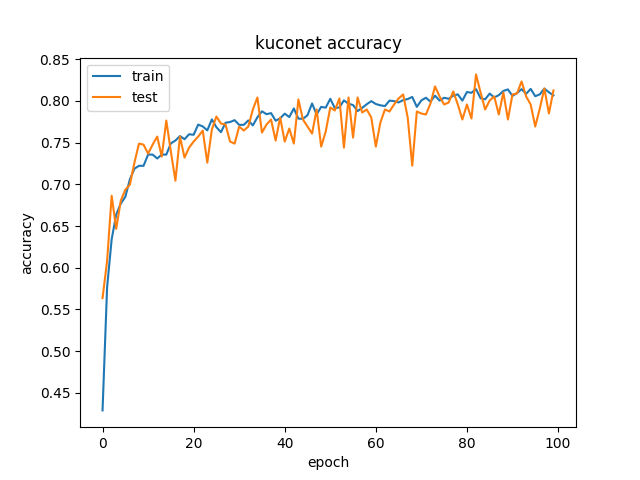
\includegraphics[width=\linewidth]{../images/kuconet_100_epochs_accuracy.png}
		\caption{Accuracy}
	\end{subfigure}
	\begin{subfigure}[b]{0.4\linewidth}
		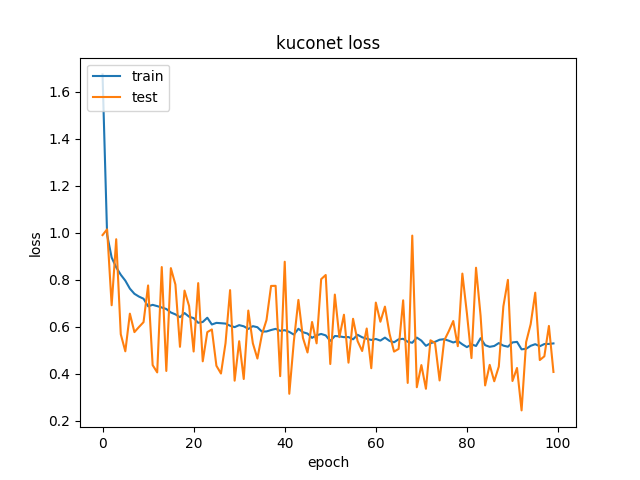
\includegraphics[width=\linewidth]{../images/kuconet_100_epochs_loss.png}
		\caption{Loss}
	\end{subfigure}
	\caption{MyNet v.1 performaces plots}
	\label{fig:mynet1performances}
\end{figure}

\subsection{KucoNet v.2}
The second CNN is defined as follow:
\begin{table}[H]
	\begin{center}
		\begin{tabular}{|l|r|}
			\hline
			\textbf{Layer (type)} & \textbf{Parameters} \\
			\hline
			Convolutional & 56, kernel $3 \times 3$ \\
			\hline
			Max Pooling & pool $2 \times 2$ \\
			\hline
			Convolutional & 32, kernel $3 \times 3$ \\
			\hline
			Max Pooling & pool $2 \times 2$ \\
			\hline
			Flatten & \\
			\hline
			Fully Connected & 64 neurons  \\
			\hline
			Fully Connected & 4 neurons \\
			\hline 
		\end{tabular}
	\end{center}
\end{table}
The first convolutional layer produces 56 feature maps using a $3 \times 3$ kernel followed by max-pooling operation. The second convolutional layer produces 32 feature maps using a $3 \times 3$ kernel followed by a max-pooling operation. After that, feature maps are sent to the dense layer, which includes 64 neurons. Finally, the last layer is a dense layer  composed by 4 neurons that produces the output. The activation function is \textit{relu} for all the layers, except the last one that uses \textit{softmax}.  The model is compiled with the \textit{Adam} optimizer and the \textit{categorical\_crossentropy} loss function. \\
\textbf{Parameters}:
\begin{itemize}
	\item Total params: 3,114,628
	\item Trainable params: 3,114,628
	\item Non-trainable params: 0
\end{itemize}
\textbf{Results}:
\begin{itemize}
	\item Final epoch performances:
	\begin{itemize}
		\item Accuracy: 0.8247
		\item Loss: 0.4534
	\end{itemize}
	\item Test set performances
	\begin{itemize}
		\item Accuracy : 0.7993
		\item Loss: 0.6309
	\end{itemize}
	\item Training time: $\approx$ 56 minutes
\end{itemize}
\begin{figure}[H]
	\centering
	\begin{subfigure}[b]{0.4\linewidth}
		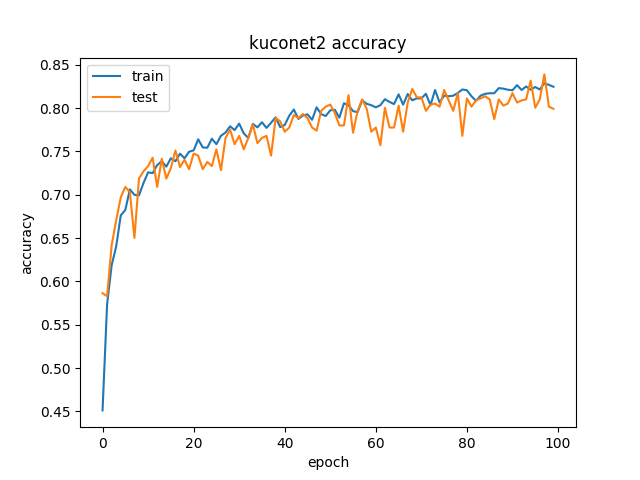
\includegraphics[width=\linewidth]{../images/kuconet2_100_epochs_accuracy.png}
		\caption{Accuracy}
	\end{subfigure}
	\begin{subfigure}[b]{0.4\linewidth}
		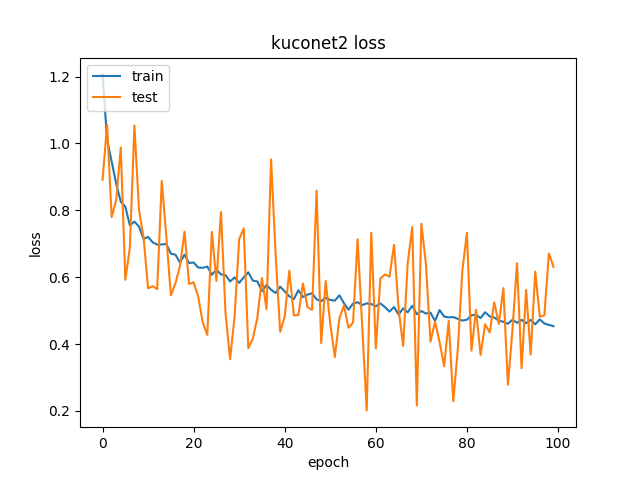
\includegraphics[width=\linewidth]{../images/kuconet2_100_epochs_loss.png}
		\caption{Loss}
	\end{subfigure}
	\caption{MyNet v.2 performaces plots}
	\label{fig:mynet2performances}
\end{figure}

\subsection{KucoNet v.3}
The third CNN is defined as follow:
\begin{table}[H]
	\begin{center}
		\begin{tabular}{|l|r|}
			\hline
			\textbf{Layer (type)} & \textbf{Parameters} \\
			\hline
			Convolutional & 32, kernel $3 \times 3$ \\
			\hline
			Max Pooling & pool $2 \times 2$ \\
			\hline
			Convolutional & 64, kernel $2 \times 2$ \\
			\hline
			Max Pooling & pool $2 \times 2$ \\
			\hline
			Flatten & \\
			\hline
			Fully Connected & 256 neurons  \\
			\hline
			Fully Connected & 4 neurons \\
			\hline 
		\end{tabular}
	\end{center}
\end{table}
The first convolutional layer produces 32 feature maps using a $3 \times 3$ kernel followed by max-pooling operation. The second convolutional layer produces 64 feature maps using a $2 \times 2$ kernel followed by a max-pooling operation. After that, feature maps are sent to the dense layer, which includes 256 neurons. Finally, the last layer is a dense layer  composed by 4 neurons that produces the output. The activation function is \textit{relu} for all the layers, except the last one that uses \textit{softmax}.  The model is compiled with the \textit{Adam} optimizer and the \textit{categorical\_crossentropy} loss function. \\
\textbf{Parameters}:
\begin{itemize}
	\item Total params: 27,076,804
	\item Trainable params: 27,076,804
	\item Non-trainable params: 0
\end{itemize}
\textbf{Results}:
\begin{itemize}
	\item Final epoch performances:
	\begin{itemize}
		\item Accuracy: 0.8087
		\item Loss: 0.5324
	\end{itemize}
	\item Test set performances
	\begin{itemize}
		\item Accuracy : 0.8257
		\item Loss: 0.7442
	\end{itemize}
	\item Training time: $\approx$ 54,5 minutes
\end{itemize}
\begin{figure}[H]
	\centering
	\begin{subfigure}[b]{0.4\linewidth}
		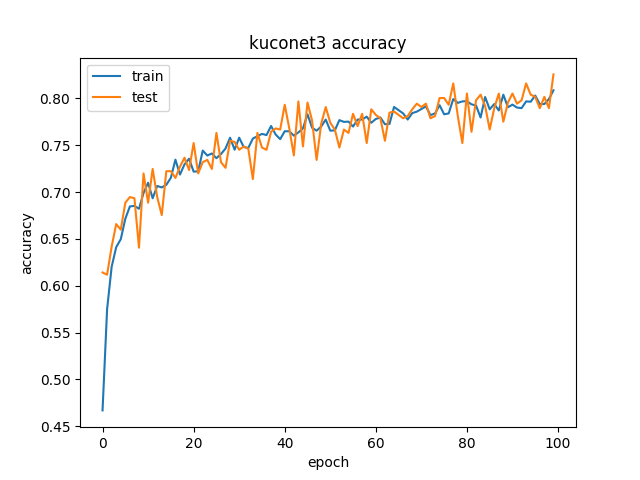
\includegraphics[width=\linewidth]{../images/kuconet3_100_epochs_accuracy.png}
		\caption{Accuracy}
	\end{subfigure}
	\begin{subfigure}[b]{0.4\linewidth}
		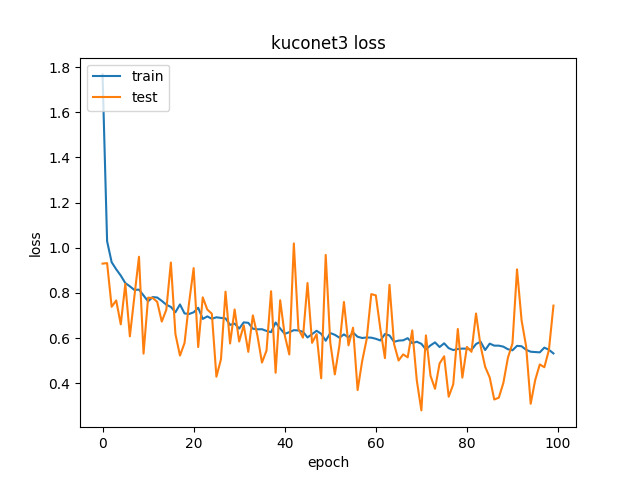
\includegraphics[width=\linewidth]{../images/kuconet3_100_epochs_loss.png}
		\caption{Loss}
	\end{subfigure}
	\caption{MyNet v.3 performaces plots}
	\label{fig:mynet3performances}
\end{figure}

\section{Transfer Learning with fine tuning}
For this task I used a \textbf{\textit{VGG16}} net pre-trained on \textit{imagenet}. I loaded the pre-trained model without the last layer (\textit{output}) and I added some new layers: a Global Average Pooling layer, a Fully Connected layer composed by 100 neurons and a Fully Connected layer of 4 neurons. Also in this case the activation function is \textit{relu} for middle layersand \textit{softmax} for the output layer. The model is compiled with the \textit{Adam} optimizer and the \textit{categorical\_crossentropy} loss function.  \\
\textbf{Parameters}:
\begin{itemize}
	\item Total params: 14,766,392
	\item Trainable params: 13,030,904
	\item Non-trainable params: 1,735,488
\end{itemize}
\textbf{Results}:
\begin{itemize}
	\item Final epoch performances:
	\begin{itemize}
		\item Accuracy: 0.9859
		\item Loss: 0.0433
	\end{itemize}
	\item Test set performances
	\begin{itemize}
		\item Accuracy : 0.8810
		\item Loss: 0.9003
	\end{itemize}
	\item Training time: $\approx$ 2 hours and 15 minutes
\end{itemize}
\begin{figure}[H]
	\centering
	\begin{subfigure}[b]{0.4\linewidth}
		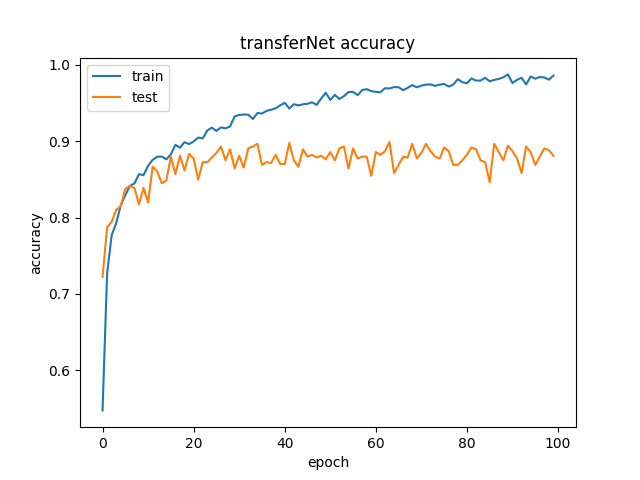
\includegraphics[width=\linewidth]{../images/transfernet_100_epochs_accuracy.png}
		\caption{Accuracy}
	\end{subfigure}
	\begin{subfigure}[b]{0.4\linewidth}
		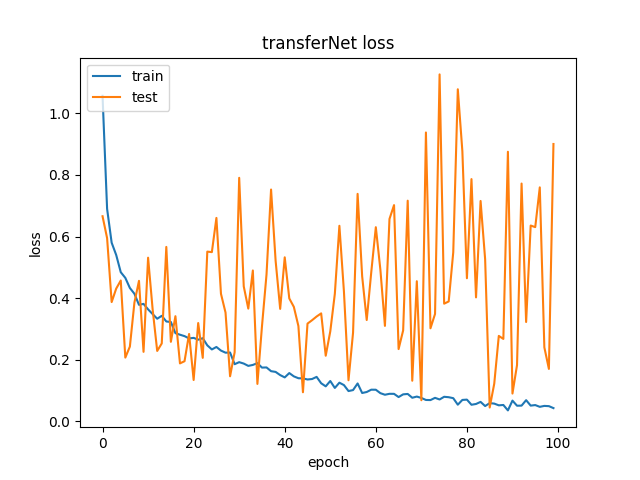
\includegraphics[width=\linewidth]{../images/transfernet_100_epochs_loss.png}
		\caption{Loss}
	\end{subfigure}
	\caption{TransferNet performaces plots}
	\label{fig:transfernetperformances}
\end{figure} \newpage
\section{Testing on other datasets}
All the nets were tested on \textit{SMART-I Weather Dataset} and my personal dataset named \textit{Kuco Dataset}. Finally I used the \textit{TransferNet} model for prediction.
\subsection{SMART-I Weather Dataset}
Testing the nets on this dataset I had the following results:
\begin{table}[H]
	\begin{center}
		\begin{tabular}{|p{0.4\textwidth}|p{0.4\textwidth}|}
			\hline
			\textbf{Net} & \textbf{Performances} \\
			\hline
			AlexNet & Accuracy: 0.331797 \\
			\cline{2-2}
					& Loss: 2.828256 \\
			\hline
			KucoNet v.1 & Accuracy: 0.478934 \\
			\cline{2-2}
						& Loss: 1.728153 \\
			\hline
			KucoNet v.2 & Accuracy: 0.499671 \\
			\cline{2-2}
						& Loss: 1.944088 \\
			\hline
			KucoNet v.3 & Accuracy: 0.455563 \\
			\cline{2-2}
						& Loss: 3.439912 \\
			\hline
			TransferNet & Accuracy: 0.598420 \\
			\cline{2-2}
						& Loss: 2.567181 \\
			\hline
		\end{tabular}
	\end{center}
\end{table}
It's possible to see how all the nets perform terribly on this dataset.


\subsection{Kuco Dataset}
This dataset is composed by some personal photos. I tried to create a balanced dataset (5 images for each class), but unfortunately I had only one rainy photo. I tested all the networks on this dataset and got the following results: \\
\begin{table}[H]
	\begin{center}
		\begin{tabular}{|p{0.4\textwidth}|p{0.4\textwidth}|}
			\hline
			\textbf{Net} & \textbf{Performances} \\
			\hline
			AlexNet & Accuracy: 0.437500 \\
			\cline{2-2}
					& Loss: 1.581957 \\
			\hline
			KucoNet v.1 & Accuracy: 0.25 \\
			\cline{2-2}
						& Loss: 1.615923 \\
			\hline
			KucoNet v.2 & Accuracy: 0.375 \\
			\cline{2-2}
						& Loss: 2.081731 \\
			\hline
			KucoNet v.3 & Accuracy: 0.5625 \\
			\cline{2-2}
						& Loss: 1.726111 \\
			\hline
			TransferNet & Accuracy: 0.5 \\
			\cline{2-2}
						& Loss: 4.648948 \\
			\hline
		\end{tabular}
	\end{center}
\end{table}
Surprisingly, \textit{KucoNet v.3} performed better than \textit{TransferNet}, and \textit{AlexNet} better than \textit{KucoNet v.1} and \textit{KucoNet v.2}

\subsection{WeatherBlindTestSet prediction}
I used the \textit{TransferNet} model to perform the prediction on \textit{WeatherBlindTestSet Dataset}. In attachment is provided the output \textit{.csv} file. 321 images were classified as \textit{SUNNY}, 502 as \textit{SNOWY}, 259 as \textit{HAZE} and 418 as \textit{RAINY}.

\section{Conclusions}
Let's summarize the results in a compact way: \\
\begin{table}[H]
	\begin{center}
		\begin{tabular}{|p{0.2\textwidth}|p{0.2\textwidth}|p{0.2\textwidth}|p{0.25\textwidth}|}
			\hline
			\textbf{Net} & \textbf{Accuracy} & \textbf{Loss} & \textbf{Training time} \\
			\hline
			AlexNet & 0.7320 & 0.9699 & $\approx$ 1h:5m \\
			\hline
			KucoNet v.1 & 0.8066 & 0.5284 & $\approx$ 1h:33m \\
			\hline
			KucoNet v.2 & 0.7993 & 0.4534 & $\approx$ 56m \\
			\hline
			KucoNet v.3 & 0.8257 & 0.7442 & $\approx$ 54,5m \\
			\hline
			TransferNet & 0.8810 & 0.9003 & $\approx$ 2h:15m \\
			\hline
		\end{tabular}
	\end{center}
\end{table}
It's easy to see that all \textit{KucoNets} perform almost the same way (each of them performs better than \textit{AlexNet} but worst than \textit{TransferNet}). The \textit{TransferNet} model has the best accuracy, but the loss is higher than the other nets. Moreover, it required much more time for training. From the graphs it is also possible to highlight how loss is very unstable in time for all the nets. \textit{KucoNet v.3} performs better than the other two, having the lower training time.

After all these considerations it is possible to conclude that solve an image classification problem based on the weather condition is a very difficult task.

\end{document}